\documentclass{standalone}
\usepackage{pgf,tikz}

\begin{document}
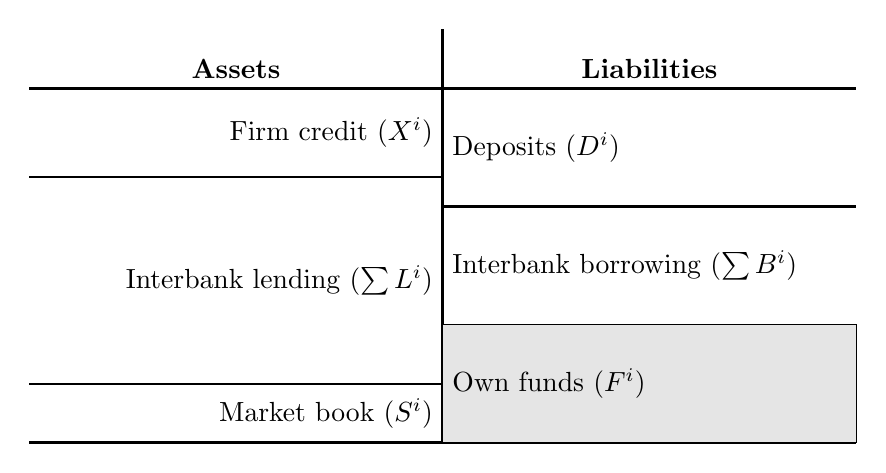
\begin{tikzpicture}[scale = 0.75]
%\draw [very thin, color = gray](0, 0) grid (14, 7);
\draw [very thick] (0, 6) to (14, 6);
\draw [very thick] (7, 7) to (7, 0);
\node [above] at (10.5, 6) {\textbf{Liabilities}};
\node [above] at (3.5, 6) {\textbf{Assets}};
\node [right] at (7, 5) {Deposits $(D^{i})$};
\draw [thick] (7,4) to (14,4);
\node [left] at (7, 5.25) {Firm credit $(X^{i})$};
\draw [thick] (0,4.5) to (7,4.5);
\node [right] at (7, 3) {Interbank borrowing $(\sum B^{i})$};
\draw [thick] (7,2) to (14,2);
\node [left] at (7, 2.75) {Interbank lending $(\sum L^{i})$};
\draw [thick] (0,1) to (7,1);
\draw [very thick] (0, 0) to (14, 0);
\node [left] at (7, 0.5) {Market book $(S^{i})$};
\draw [fill=gray!20] (7,0) rectangle (14,2);
\node [right] at (7, 1) {Own funds $(F^{i})$};
\end{tikzpicture}
\end{document}

